% !TEX root = main.tex

\documentclass[a4paper, UKenglish, 11pt]{uiomaster}
\usepackage{lipsum}
\usepackage[subpreambles=true]{standalone}

\begin{document}

\chapter{Introduction to Neuroscience} \label{chap:intro_neuro}

% Source for the first sentence ?
Neuroscience is a multidisciplinary field focused on understanding the complexities of the human brain and nervous system. At its core, neuronal communication forms the foundation for brain function, where billions of neurons interact through electrical signals. Electroencephalography (EEG) plays a pivotal role in recording and analyzing the electrical communication in the brain. Most importantly EEG serves as a non-invasive tool to detect abnormal brain activity and identify neurological disorders such as epilepsy. By exploring electrical brain activity, neuroscience aim to advance our comprehension of the human brain and improve diagnostic and therapeutic approaches for various neurological conditions.

In this introductory chapter, we will delve into the foundational aspects of neuronal communication, which will be usefull in chapter 2, where we will explore the principles of EEG recordings. By familiarizing ourselves with the fundamental concepts of neurons, we hope to gain a deeper understanding of the applications of EEG in the dynamic field of neuroscience. The chapter is based on the books "Neuronal Dynamics" by Gerstner, Kistler, Naud, and Paninski \cite{gerstner2014neuronal} and "Principles of Computational Modelling in Neuroscience" by Sterratt, Graham, Gillies, and Willshaw \cite{sterratt2011principles}.

% Exitatory and inhibatory !!

% NEW IDEAS:
% Final section: abnormal electrical signals, recordings, eeg --- will introduce in next chapter

\section{The Neuron}

Neurons are the fundamental units of the central nervous system, forming intricate networks with numerous interconnections. Similar to other cells, neurons have a voltage difference across their cell membrane known as the membrane potential. This membrane potential is a result of the selective permeability of the cell membrane to different ions, particularly sodium (Na+), calcium (Ca2+), and chloride (Cl-). At rest, the neuron maintains a relatively higher concentration of sodium ions outside the cell and a higher concentration of potassium ions inside the cell. This difference in ion concentrations, along with the presence of ion channels that regulate the flow of ions in and out of the cell, contributes to the resting membrane potential. Typically, the membrane potential of a neuron hovers around -65 mV, indicating that the interior of the cell is negatively charged compared to the external environment \cite{sterratt2011principles}.

A neuron consists of three distinct parts: the \emph{dendrites}, the \emph{soma}, and the \emph{axon}. Dendrites, with their branching structure, play an important role in collecting signals from other neurons. These signals are transmitted to the soma, which acts as the central processing unit, performing essential nonlinear processing. If the total input received by the soma reaches a specific threshold, an \emph{action potential} is initiated. This signal generates an electrical current that travels along the axon. When the electrical current reaches the \emph{synaptic cleft}, chemical messengers known as \emph{neurotransmitters} are realised. These messengers play the key role in transmitting the signal to the next neuron. If \emph{receptors} on the receiving neuron accept the neurotransmitters, a new electrical signal is generated. This transmission of signals between neurons the synapses is called \emph{synaptic input} \cite{gerstner2014neuronal}.

In Figure \ref{fig:neuron}, we have provided a basic illustration of a single neuron with dendrites, soma, and axon.

\begin{figure}
    \centering
    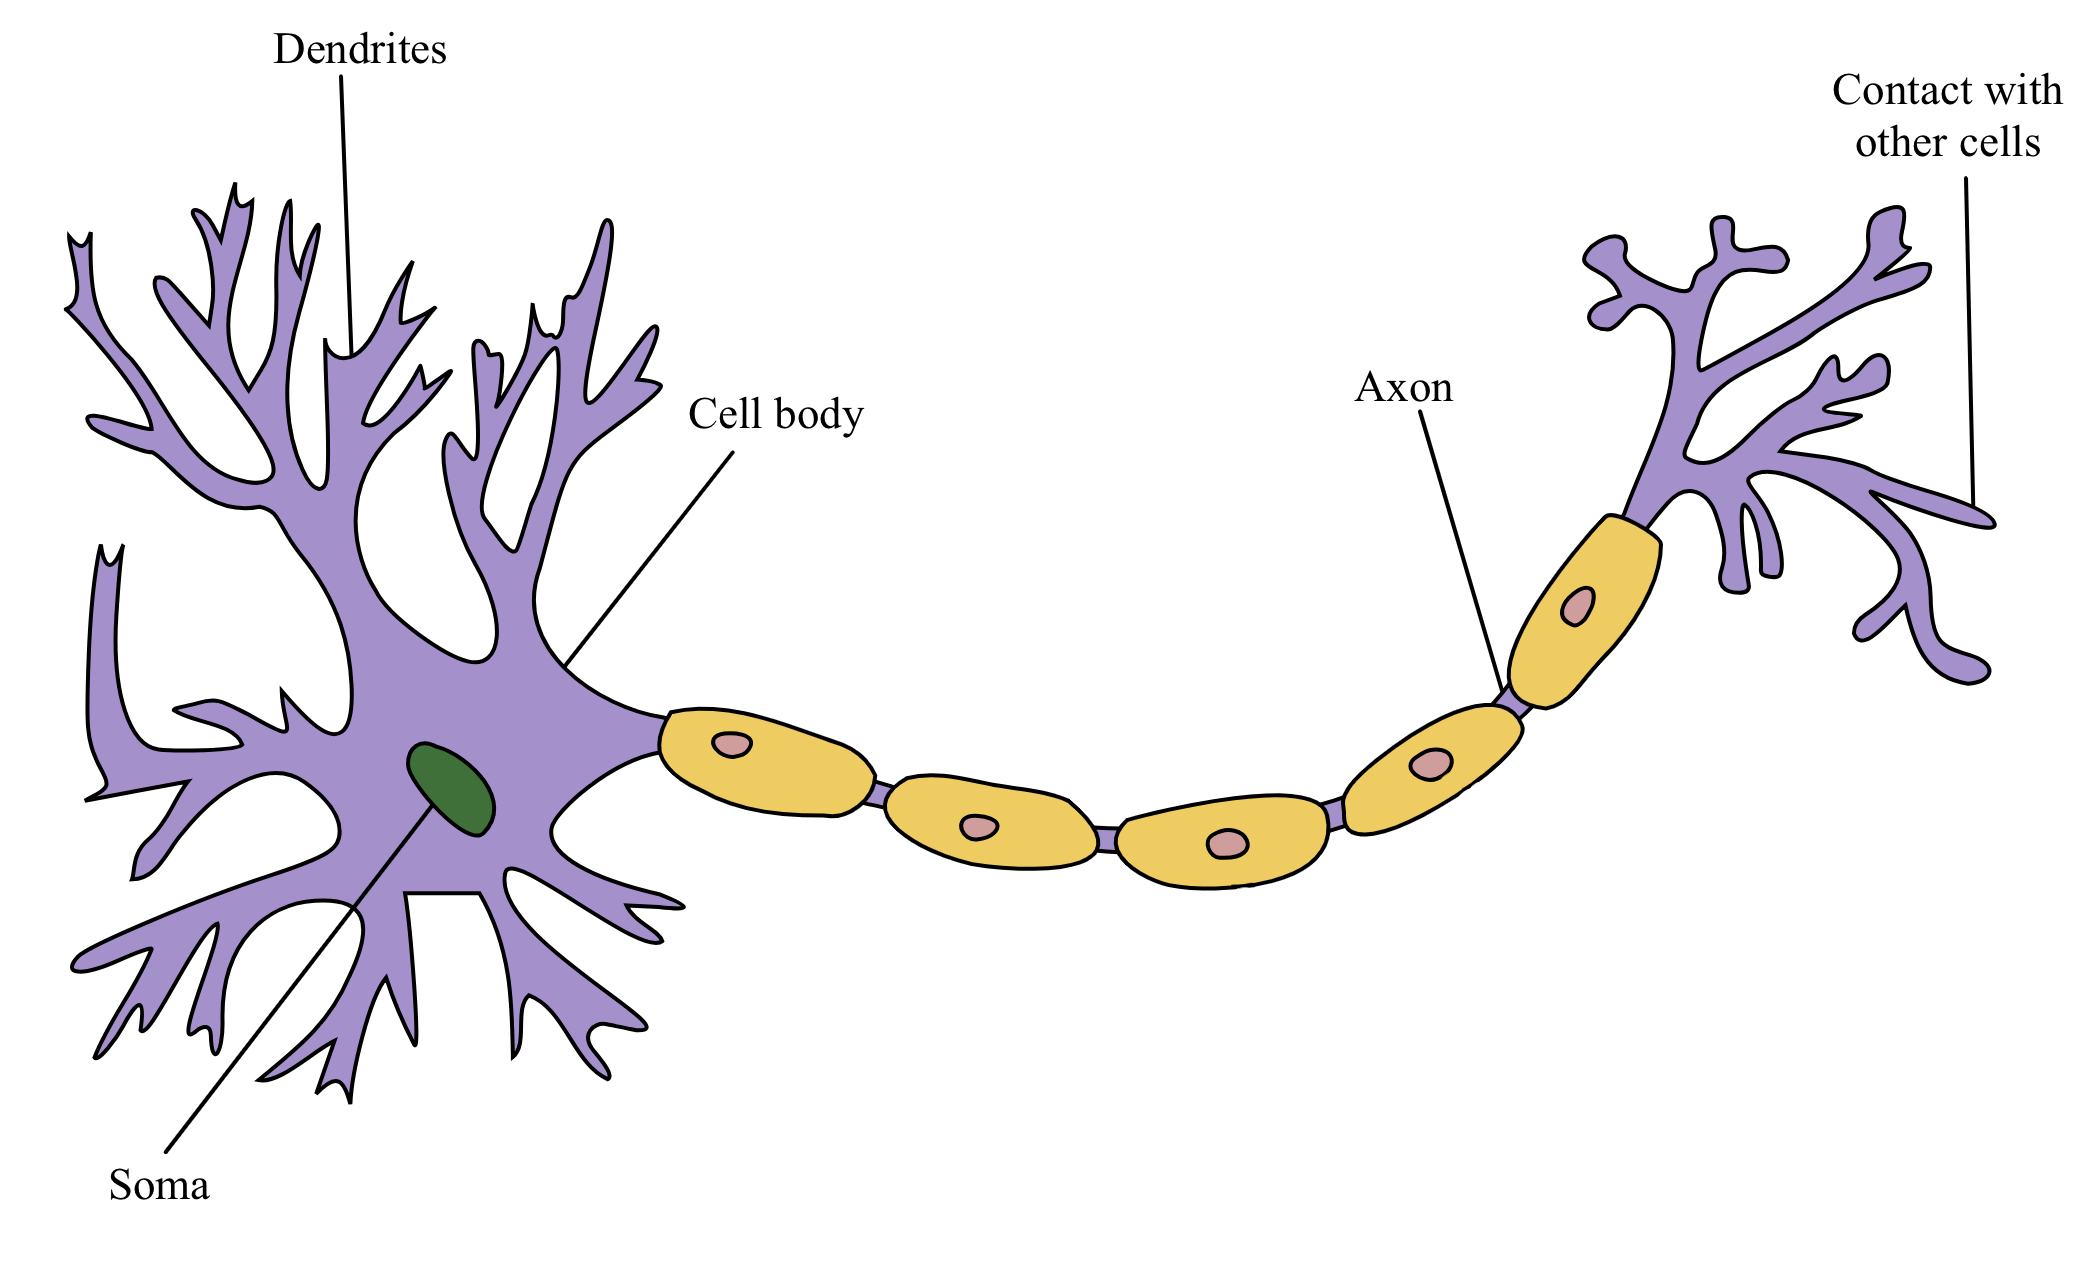
\includegraphics[width=1.0\linewidth]{figures/Neuron_wikimedia.png}
    \caption{Illustation of single neuron with dendrites, soma and axon. The figure has been adapted from Wikimedia Commons with attribution to Quasar Jarosz at English Wikipedia and is licensed under the Creative Commons Attribution-Share Alike 3.0 Unported license \cite{wikimedia-neuron}. The figure has been edited to remove some of the original details.}
    \label{fig:action_potential}
\end{figure}


% \subsection{Some title leadning to EEG abnormal shape }
\section{Spike Trains and Action Potentials}
\rednote{Fix illustation so that it does not contain depolarization, repolarization and refractory period?}

When the electrical signals transmitted towards the soma reach the so-called threshold value, usually around -55 mV, the neuron fires. This initiation of an action potential, when observed in intracellular recordings, can be seen as a spike with an amplitude of about 100 mV and a duration of 1-2 ms \cite{gerstner2014neuronal}. In Figure \ref{fig:action_potential}, we have provided an illustration of the typical intracellular action potential.


\begin{figure}
    \centering
    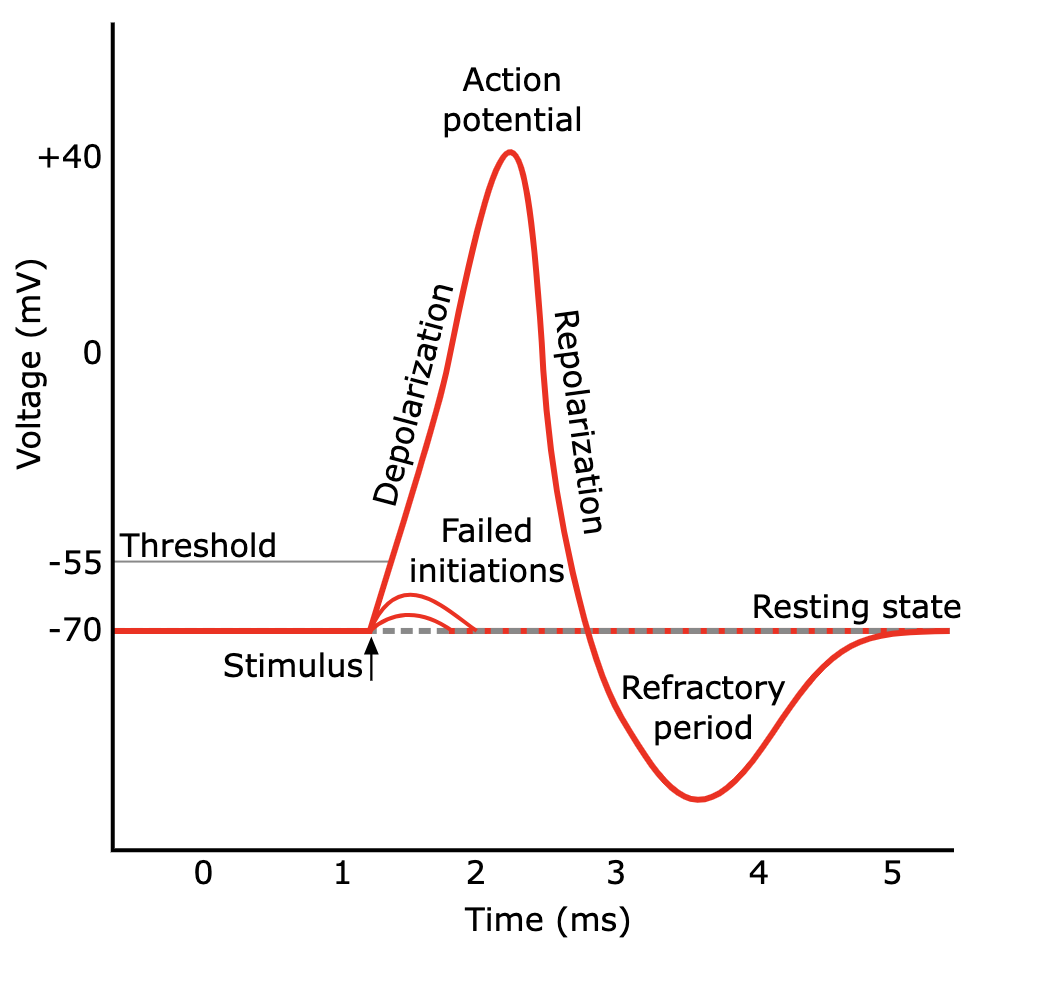
\includegraphics[width=0.8\linewidth]{figures/action_potential.png}
    \caption{Illustation of a characteristic action potential. The figure have been adapted from Wikimedia Commons and are licensed under the Creative Commons Attribution-Share Alike 3.0 Unported license \cite{wikimedia-action}. The figure has been edited to remove some of the original details.}
    \label{fig:action_potential}
\end{figure}

The action potential is characterised by a swift and steep rise in the electrical potential, resulting in a rapid upward, positive spike, followed by a quick decline in the potential back to the resting state. This form of the action potentials remains relatively constant throughout the propagation along the axon. When collecting information out of these spikes, it is therefor not the shape of the spikes that is studied. Instead, the information lies in the number and timing of chains of action potentials emmitted by the neuron, also reffered to as \emph{spike trains}.

Spike trains observed during epileptic seizures exhibit distinguishable characteristics compared to spike trains in regular neural activity. Epileptic seizures result from bilateral synchronous firing of neurons and manifest as specific EEG patterns known as \emph{spike-and-wave discharges}. These discharges exhibit repetitive and rhythmic patterns, typically occurring at a frequency of around 2.5 Hz, setting them apart from the irregular and asynchronous firing of action potentials seen in typical spike trains\cite{gerstner2014neuronal}. During epileptic events, the initiation of spike-and-wave discharges involves complex mechanisms, including the interplay of voltage-gated sodium and calcium channels and the role of inhibitory postsynaptic potentials \cite{wiki:electroencephalography}. \rednote{Wikipedia citation. See if I can use Torbjørn book instead.}
%This stark contrast in the rhythmicity and temporal dynamics of epileptic spike trains highlights the distinct nature of epileptic activity when compared to the more variable and less periodic patterns observed in "normal" neuronal firing \cite{gerstner2014neuronal}.

% Need to be rewritten somehow.
% The hypersynchronous discharges that occur during a seizure may begin in a very discrete region of cortex and then spread to neighboring regions. Seizure initiation is characterized by two concurrent events: 1) high-frequency bursts of action potentials, and 2) hypersynchronization of a neuronal population. The synchronized bursts from a sufficient number of neurons result in a so-called spike discharge on the EEG. At the level of single neurons, epileptiform activity consists of sustained neuronal depolarization resulting in a burst of action potentials, a plateau-like depolarization associated with completion of the action potential burst, and then a rapid repolarization followed by hyperpolarization. This sequence is called the paroxysmal depolarizing shift. (Slide 23) The bursting activity resulting from the relatively prolonged depolarization of the neuronal membrane is due to influx of extracellular Ca++, which leads to the opening of voltage-dependent Na+ channels, influx of Na+, and generation of repetitive action potentials. The subsequent hyperpolarizing afterpotential is mediated by GABA receptors and Cl− influx, or by K+ efflux, depending on the cell type.

% spike-and-vale / epileptiform activity  ... can be measured on eeg recordings... blabla .... spike trains looks like for epilepsy ... can be picked up on eeg recordings
% MAYBE NOT INCLUDE anything about eeg here, if anything, include how one can pick up on abnormal activity  ??

\section{Anatomy of the Cortex}
\rednote{Fill in from sources, paper etc. https://www.cell.com/current-biology/pdf/S0960-9822(11)01198-5.pdf, https://www.ncbi.nlm.nih.gov/books/NBK2510/}
% Taken from the book and need to be rewritten !
Neurons in the brain are part of a vast network, interwoven with billions of other neurons and glial cells, creating the complex brain tissue. The brain is divided into various regions, and one essential area is the cortex, a thin but expansive sheet of neurons that folds over other brain structures. Different cortical areas have specific roles; some are specialized in processing sensory information, while others handle working memory or control motor functions \cite{gerstner2014neuronal}.

The human cerebral cortex is typically divided into six layers. The oldest part of the cortex, known as the archipallium, has a more straightforward structure with three distinct neuronal layers. Within the archipallium, the hippocampus plays a major role in learning and memory functions. It is a crucial cortical structure implicated in the development of some common epilepsy syndromes \cite{bromfield2006introduction}.

Neurons communicate through synapses, where \emph{presynaptic neurons} sends, and \emph{postsynaptic cells} receives the electrical signals. In the animal brain, a single presynaptic neuron can connect to over 10,000 postsynaptic neurons. While many axonal branches end close to the neuron itself, some axons extend several centimeters to reach neurons in other brain regions \cite{gerstner2014neuronal}.

Within the cortex, there are two primary classes of neurons. \emph{Pyramidal neurons} send information to distant areas of the brain, and play a crucial role in long-distance communication. On the other hand, \emph{interneurons} are considered local-circuit neurons, exerting their influence on nearby neurons. Most pyramidal neurons form excitatory synapses, meaning they stimulate post-synaptic neurons, while most interneurons form inhibitory synapses, meaning they suppress the activity of pyramidal cells or other inhibitory neurons \cite{bromfield2006introduction}.


% \section{Head Models and Multicompartmental Modeling }
% % Something more about volume conducters
%
% \section{Currents and Potentials in the Brain}
% Ohm's law in volume conductors is a more genral statement than its usual form in electrical circuits. It is a linear relationship between vector current density $J$ and the electric field $E$. The law is then expessed as follows:
%
% \begin{equation}
% J = \sigma E,
% \label{eq:ohms_law}
% \end{equation}
%
% where $\sigma$ is the conductivity of the .... (physical material). (Soruce: Electric Fields of the Brain: The Neurophysics of EEG).


% \rednote{rewrite}
% When a single pyramidal cell is stimulated and reaches its threshold, it generates an action potential. During this process, the synapse receives an excitatory signal, leading to a post-synaptic potential where positively charged ions enter the cell. As a result, a relatively negative charge is induced in the nearby extracellular space, which refers to the fluid-filled space surrounding the neuron. As the electrical signal travels down the dendrite, it eventually exits the cell membrane at locations further away from the synapse, and these locations are referred to as the "source." Consequently, an outward flow of positive charge prevails, leading to a relatively positive charge in the extracellular space. This spatial configuration creates an external dipole, with a relatively negative charge at the distant part of the dendrite and a positive charge closer to the cell body \cite{bromfield2006introduction}.


\end{document}